% Chapter Template

\chapter{Mapping and Scheduling} % Main chapter title

\label{c:sched} % Change X to a consecutive number; for referencing this chapter elsewhere, use \ref{ChapterX}

%----------------------------------------------------------------------------------------
%	SECTION 1
%----------------------------------------------------------------------------------------

	The two mode AMC response time analysis for mixed criticality systems was presented in Section~\ref{s:mixedcriticality}. 
	We have shown that it is advantageous to consider a four mode model when both transient faults and execution time overruns are possible in a single lockstep-core mixed criticality fault tolerant system (MCFTS) \cite{albayati2016modes}. 
	This chapter will review the four mode analysis and initial single core results on improved quality of service (QoS) and then extend it to include several ODR strategies in multicore systems. 
	A DSE mapping algorithm that uses the new analysis will then be presented.

\section{Four Mode MCFTS Model}
\label{s:mcfts}
	AMC response time analysis depends on the notion that safety critical systems must be proven operational under optimistic and pessimistic worst case execution time estimates. 
	A runtime mechanism must be available to monitor the execution time of tasks in the system.
	Some or all LO tasks must be dropped from the system when a any task overruns its optimistic execution time budget.
	In order to accomodate fault tolerance, we extend the analysis to scenarios where a task may also execute more than once in case of failure.
	
	Initial work on AMC assumed that all LO tasks are dropped during a mode change. 
	Current work in MCS aims to reduce the amount of LO criticality tasks that must be dropped through migration in multicore systems \cite{al2015enhanced} and designer specified importance \cite{fleming2014incorporating}. 
	We introduce a four mode model to MCFTS in order to reduce the number of LO tasks that must be dropped in the event that only an execution overrun or transient fault occurs rather than both. 
	We initially consider a lockstep core that is capable of detecting but not correcting errors.
	The RTOS kernel is assumed to remain uncorrupted.
	Under these conditions, a task may be re-executed when an error is detected.
		The four modes intuitively improve QoS because any response time analysis that considers both faults and overruns at the same time will be overly pessimistic in deciding which tasks to drop.
	\addfigure{0.6}{modes.pdf}{The 4 modes of operation in MCFTS analysis.}{f:modes}
\addfigure{0.6}{sched-example.pdf}{Mode change scenarios.}{f:mode-scenarios}
	
	The four modes and their transition conditions are shown in Figure~\ref{f:modes}. 
	Initially, the system is in LO mode. 
	When a transient fault is detected, the system transitions into TF mode. 
	If an execution overrun occurs ($C>C(LO)$), then the system transitions into OV mode. 
	Finally, a transition to HI mode occurs from one of the intermediate mode if the other event occurs before a transition back to LO mode.\footnote{Reverse transitions are usually treated as a separate problem in MCS and is not considered in this thesis. Possible implementation may be found in \cite{bate2015bailout}.}
	
	Three example scenarios are presented in Figure~\ref{f:mode-scenarios} for the task set in Table~\ref{t:example}. 
	In scenario (a), $\tau_1$ exceeds its $C(LO)$ threshold of 3 and the system transitions into OV mode. In scenario (b), $\tau_1$ suffers a transient fault and required re-execution. The system stays in TF mode because none of the re-executions exceed $C(LO)$. In scenario (c), $\tau_1$ first exceeds $C(LO)$ and the system transitions to OV mode. Once in OV mode, an fault occurs and the system transitions into HI mode, presumably dropping even more tasks.
	

	
	
\subsection{Response Time Analysis}
	
	
	\begin{table}[t!]
\caption{Example Task Set}
\centering

	\begin{tabular}{@{}lcccc@{}}
	\toprule
	& $C(LO)$ & $C(HI)$ & T=D & L 	 \\
	\bottomrule
	$\tau_1$ & 3 & 4 & 12 & HI  \\
	$\tau_2$ & 4 & - & 12 & LO  \\
	$\tau_3$ & 4 & - & 12 & LO  \\
	$\tau_4$ & 1 & - & 12 & LO  \\
	\end{tabular}

\label{t:example}
\end{table}
	
	%In addition to the LO and HI modes, there is now a transient fault (TF) and overrun (OV) mode. 
	Equations \ref{eq:lomode}-\ref{eq:hiovmode} show the updated four mode response time analysis.
	
	
\begin{equation}
R_i^{(LO)}= C_i(LO)+\sum_{j \in hp(i)}\Big\lceil\frac{R_i^{(LO)}}{T_j}\Big\rceil \cdot C_j(LO)
\label{eq:lomode}
\end{equation}

\begin{equation}\label{eq:ovmode}
\begin{aligned}
R_i^{(OV)} &  = C_i(L_i)+\sum_{j \in hpC(OV,i)}\Big\lceil\frac{R_i^{(OV)}}{T_j}\Big\rceil \cdot C_j(L_j) 
 +\sum_{k \in hp(i)-hpC(OV,i)}\Big\lceil\frac{R_i^{(LO)}}{T_k}\Big\rceil \cdot C_k(LO)
\end{aligned}
\end{equation}
	
	
	The LO mode analysis remains unchanged. Equation~\ref{eq:ovmode} shows the response time for the OV mode. 
	The set of tasks $hpC(L,i)$ is defined as the set of tasks with higher priority than $\tau_i$ that are not dropped in mode $L$. 
	Therefore, in the OV mode, we can see that the jobs that continue to execute are assumed to take the maximum amount of time $C(OV)=C(HI)$ whereas the dropped jobs ($hp(i) - hpC(OV,i)$) only execute during $R_i(LO)$ for up to their $C(LO)$ times.
	
\begin{equation}\label{eq:tfmode}
\begin{aligned}
R_i^{(TF)} & = n_i(TF) \cdot C_i(LO)
+\sum_{j \in hpC(TF,i)}\Big\lceil\frac{R_i^{(TF)}}{T_j}\Big\rceil \cdot n_j(TF) \cdot C_j(LO) \\
&  +\sum_{k \in hp(i)-hpC(TF,i)}\Big\lceil\frac{R_i^{(LO)}}{T_k}\Big\rceil \cdot C_k(LO)
\end{aligned}
\end{equation}

	Equation~\ref{eq:tfmode} shows the response time for TF mode. 
	In the transient fault mode at least one task must re-execute. 
	Each task is assigned a maximum number of executions that it is required to run, $n_i$, in order to meet some threshold in terms of probability of failure (derivation in \cite{albayati2016modes}). 
	In the TF mode, the execution time is still assumed not to exceed the optimistic threshold $C(LO)$. 
	The resulting execution time for task $\tau_i$ is $n_i(TF) \cdot C_i(LO)$ where $n_i$ is the number of re-executions required in the TF mode.\footnote{$n$ depends on $C$, therefore it is possible that $n(TF) \ne n(HI)$ though this is not often the case.}

	Finally, Equations~\ref{eq:hiovmode} and \ref{eq:hitfmode} show the response time analysis for transitions from OV to HI and TF to HI modes, respectively. The set of dropped jobs on the final transition is different for the two modes.





\begin{equation}\label{eq:hiovmode}
\begin{aligned}
R_i^{(HI-OV)} & = n_i(HI) \cdot C_i(L_i) 
  +\sum_{j \in hpC(HI,i)}\Big\lceil\frac{R_i^{(HI-OV)}}{T_j}\Big\rceil \cdot n_j(HI) \cdot C_j(L_j) \\
&  +\sum_{k \in hpC(OV,i)-hpC(HI,i)}\Big\lceil\frac{R_i^{(OV)}}{T_k}\Big\rceil \cdot C_k(LO) \\
& \hspace{1cm}  +\sum_{l \in hp(i)-hpC(OV,i)}\Big\lceil\frac{R_i^{(LO)}}{T_l}\Big\rceil \cdot C_l(LO)
\end{aligned}
\end{equation}

\begin{equation}\label{eq:hitfmode}
\begin{aligned}
R_i^{(HI-TF)} & = n_i(HI) \cdot C_i(L_i)
  +\sum_{j \in hpC(HI,i)}\Big\lceil\frac{R_i^{(HI-TF)}}{T_j}\Big\rceil \cdot n_j(HI) \cdot C_j(L_j) \\
&  +\sum_{k \in hpC(TF,i)-hpC(HI,i)}\Big\lceil\frac{R_i^{(TF)}}{T_k}\Big\rceil \cdot C_k(LO) \\
& \hspace{1cm}  +\sum_{l \in hp(i)-hpC(TF,i)}\Big\lceil\frac{R_i^{(LO)}}{T_l}\Big\rceil \cdot C_l(LO)
\end{aligned}
\end{equation}

\subsection{Reducing Model Pessimism}

	The model is still highly pessimistic as \emph{all} tasks are assumed to re-execute upon a transition into TF mode. 
	This pessimisim is reduced by the introduction of a new parameter $F$, the maximum number of faults expected in an interval $D_{max}$, the largest relative deadline among the tasks in the task set.
	For example, if $\tau_i$ and $\tau_j$ preempt $\tau_k$, then it is obviously beneficial when calculating the response time of $\tau_k$ that \emph{only} $\tau_i$ \emph{or} $\tau_j$ may preempt $\tau_k$ but not both.

	The term $n_i$ in the response time equations for HI and TF modes may be replaced with a new term $1 + f_i$ where $f_i$ is the maximum number of faults that may occur for task $\tau_i$. The updated equation for $R^{(TF)}$ is given by:
	\begin{equation}\label{eq:mode3new}
\begin{aligned}
R_i^{(TF)} & = (1+f_i) \cdot C_i(LO) \\
&  +\sum_{j \in hpC(TF,i)}\Big\lceil\frac{R_i^{(TF)}}{T_j}\Big\rceil \cdot (1+f_j) \cdot C_j(LO) \\
&  +\sum_{k \in hp(i)-hpC(TF,i)}\Big\lceil\frac{R_i^{(LO)}}{T_k}\Big\rceil \cdot C_k(LO)
\end{aligned}
\end{equation}
under the constraints:
\begin{subequations}
%\small
\begin{equation}
1+f_i \le n_i, \ \ fi \ge 0 \,  \forall \tau_i
\end{equation}
\begin{equation}
\sum_i{f_i} \le F.
\end{equation}
\end{subequations}

\subsection{Four Mode QoS Results for Single Core}
\label{s:singlecore-results}
	We defined QoS to be the percentage of LO criticality tasks not dropped in any given mode. The QoS for the LO mode is always 1. Random task sets were generated according to the UUnifast algorithm \cite{bini2005measuring} such that LO mode utilization is approximately 80\% on all cores. The ratio $C(HI)/C(LO)$ is determined randomly from the range $[1,2]$ and periods were chosen at random from the set ${10,20,40,50,100,200,400,500,1000}$. For each test, the average of 1000 systems is presented.

\addfigure{0.6}{final-allModesNoF.pdf}{Modes OV and TF achieve better QoS than HI for all utilizations ($F$ not bounded).}{f:util_basic}
\addfigure{0.6}{averageQoS.pdf}{Average improvement over all system utilizations for OV and TF modes compared to HI mode. }{f:avgU}

	Figure~\ref{f:util_basic} shows the QoS of OV and TF modes is improved over the HI mode for all utilizations in systems of 20 tasks (10 HI and 10 LO). LO task QoS is better in the OV and TF modes than in the HI mode. On average, the OV and TF modes outperform the HI mode by 42.9\% and 20.2\% respectively. The improvement increases with the utilization, especially for the OV mode which could be significant in systems where transient faults are less frequent than execution time overruns. Figure~\ref{f:avgU} shows the average improvement of QoS across all utilizations for the TF and OV mode compared to the HI mode.
	
\addfigure{0.6}{final-percentHI.pdf}{Modes OV and TF achieve better QoS than HI for different percentages of HI tasks ($F$ not bounded).}{f:perchi_basic}
	
	Figure~\ref{f:perchi_basic} shows a similar picture, this time holding utilization constant at 80\% while exploring the percentage of HI tasks. The QoS of the HI and TF modes degrade quickly as the percentage of HI tasks increases because none of these tasks can be dropped and the penalty for re-execution becomes very severe.
	 	
\addfigure{0.6}{TFmodeAvgu.pdf}{Performance of TF mode for different $F$}{f:avgUN}
	Figure~\ref{f:avgUN} shows how the $F$ parameter improves QoS for the TF mode ($F=\infty$ is the default). QoS improves by about 15\% compared to the default when only two errors are assumed to occur close enough in time to affect the same mode change.

\section{Extending Response Time Analysis to ODR}

	We will extend the analysis on lockstep (LS) to support three types of ODR. The four scenarios are shown in Figure~\ref{f:ftm}. 
	In (a), LS execution occurs when a node has internal mechanisms for detecting but not correcting errors. 
	An error simply results in a re-execution on that node, as previously discussed. 	
	In (b), dual modular redundancy (DMR) replicates a thread on two cores that cannot detect errors. 
	The task must be re-executed if the task executions are found not to match by some external comparison and voting mechanism.
	In (c), triple modular redundancy (TMR) replicates a thread on three cores that cannot detect errors. 
	If an error occurs, the majority answer is taken from the three replicas and no re-execution is required.
	Finally, in (d), passive replication is similar to TMR but the final replica does not execute if the first two copies return the same result. 


\addfigure{0.55}{ftm.pdf}{The 4 fault tolerance mechanisms supported by the proposed MCFTS analysis}{f:ftm}
	
	Each technique is expressed in the new analysis by three parameters: a task set transformation, mapping constraints, and a re-executiong profile denoted by $N$.
	The task set transformation represents each replica explicitly in the task set. 
	Consider the example task set in Table~\ref{t:transform}. 
	Lockstep does not introduce any replicas to the system and does not require any transformation of the task set. 
	DMR requires one replica to be added to the task set while TMR and PR require two replicas to be added.
	
	Constraints must be added to the problem for the processors $\pi_i$ assigned to $\tau_i$ in order to properly reflect the semantics of the different techniques. 
	The constraints shown in the table ensure that the replicas are not assigned to the same core. 
	These constraints will be useful in the mapping stage.
	
	
\begin{table}
\centering
\caption{Task set transformations}
\label{t:transform}
	\begin{subtable}{0.3\textwidth}
		\caption{Example task set}
		\begin{tabular}{@{}l|cccc@{}}
		\toprule
		& C(LO) & C(HI) & T=D & L 	 \\\bottomrule
		$\tau_1$ & 5 & 10 & 25 & HI  \\
		$\tau_2$ & 5 & - & 20 & LO  \\
		\multicolumn{5}{c}{ } \\
		\multicolumn{5}{c}{ } \\
		\end{tabular}
	\end{subtable} \hspace{2cm}
	\begin{subtable}{0.3\textwidth}
		\caption{DMR transformation}
		\begin{tabular}{@{}l|cccc@{}}
		\toprule
				& C(LO) & C(HI) & T=D & L	 \\\bottomrule
		$\tau_1$ & 5 & 10 & 25 & HI  \\
		$\tau_{1.1}$ & 5 & 10 & 25 & HI  \\
		$\tau_2$ & 5 & - & 20 & LO  \\
		\multicolumn{5}{c}{$\pi_1 \ne \pi_{1.1}$}
		\end{tabular}
	\end{subtable}
	
	\begin{subtable}{0.3\textwidth}
		\caption{TMR transformation}
		\begin{tabular}{@{}l|cccc@{}}
		\toprule
				& C(LO) & C(HI) & T=D & L	 \\\bottomrule
		$\tau_1$ & 5 & 10 & 25 & HI  \\
		$\tau_{1.1}$ & 5 & 10 & 25 & HI  \\
		$\tau_{1.2}$ & 5 & 10 & 25 & HI  \\
		$\tau_2$ & 5 & - & 20 & LO  \\
		\multicolumn{5}{c}{$\pi_1 \ne \pi_{1.1} \ne \pi_{1.2}$}
		\end{tabular}
	\end{subtable} \hspace{2cm}
	\begin{subtable}{0.3\textwidth}
		\caption{PR replication}
		\begin{tabular}{@{}l|cccc@{}}
		\toprule
		& C(LO) & C(HI) & T=D & L	 \\\bottomrule
		$\tau_1$ & 5 & 10 & 25 & HI  \\
		$\tau_{1.1}$ & 5 & 10 & 25 & HI  \\
		$\tau_{1.2}$ & 5 & 10 & 25 & HI  \\
		$\tau_2$ & 5 & - & 20 & LO  \\
		\multicolumn{5}{c}{$\pi_1 \ne \pi_{1.1}$}
		\end{tabular}
	\end{subtable}
\end{table}


	The re-execution variable $n_i$ has been generalized into the vector:
\begin{equation}
	N_i=<n_i(LO),n_i(OV),n_i(TF),n_i(HI)>
\end{equation} 
	The $N$ for each mode is shown in Table~\ref{t:reex} and the updated equation for the OV mode response time are given by the following equations:
	\begin{equation}
\begin{aligned}
R_i^{(OV)} =
\begin{dcases*}
C_i(L_i)\color{red} \color{black}+\sum_{j \in hpC(OV,i)}\Big\lceil\frac{R_i^{(OV)}}{T_j}\Big\rceil \cdot C_j(L_j) \\
\hspace{0.3cm} +\sum_{k \in hp(i)-hpC(OV,i)}\Big\lceil\frac{R_i^{(LO)}}{T_k}\Big\rceil \cdot C_k(LO), &  $n_i(OV)>0$ \\
	0, & $n_i(OV)=0$
\end{dcases*}
   \end{aligned}
\end{equation}
	We note that all techniques have $n(LO)$ and $n(OV)$ values of either 0 or 1. When $n=0$, the task is not executing and the response time is simply 0. The same is true for LO mode.
	
	For example, TMR has $N=<1,1,1,1>$. This means that in all modes, any task using TMR will have $n=1$ which in effect signals that no re-executions are required. For PR, one replica executes one time in all modes and the other only executes in the case of a fault (hence only executes once in TF or HI modes).

	\begin{table}
\caption{Re-execution profiles for the fault tolerance mechanisms}
\label{t:reex}
\centering
	\begin{tabular}{@{}l|c@{}}
	\toprule
	Technique & Profile ($N$) \\
	\bottomrule
	LS & $<1,2,1,2>$ \\
	DMR & $<1,2,1,2>$ \\
	TMR & $<1,1,1,1>$ \\
	PR & $<1,1,1,1>$ and $<0,1,0,1>$ \\
	\end{tabular}
\end{table} 	

\section{Design Space Exploration}

\subsection{Genetic Algorithm}
\begin{figure}[h]
\centering
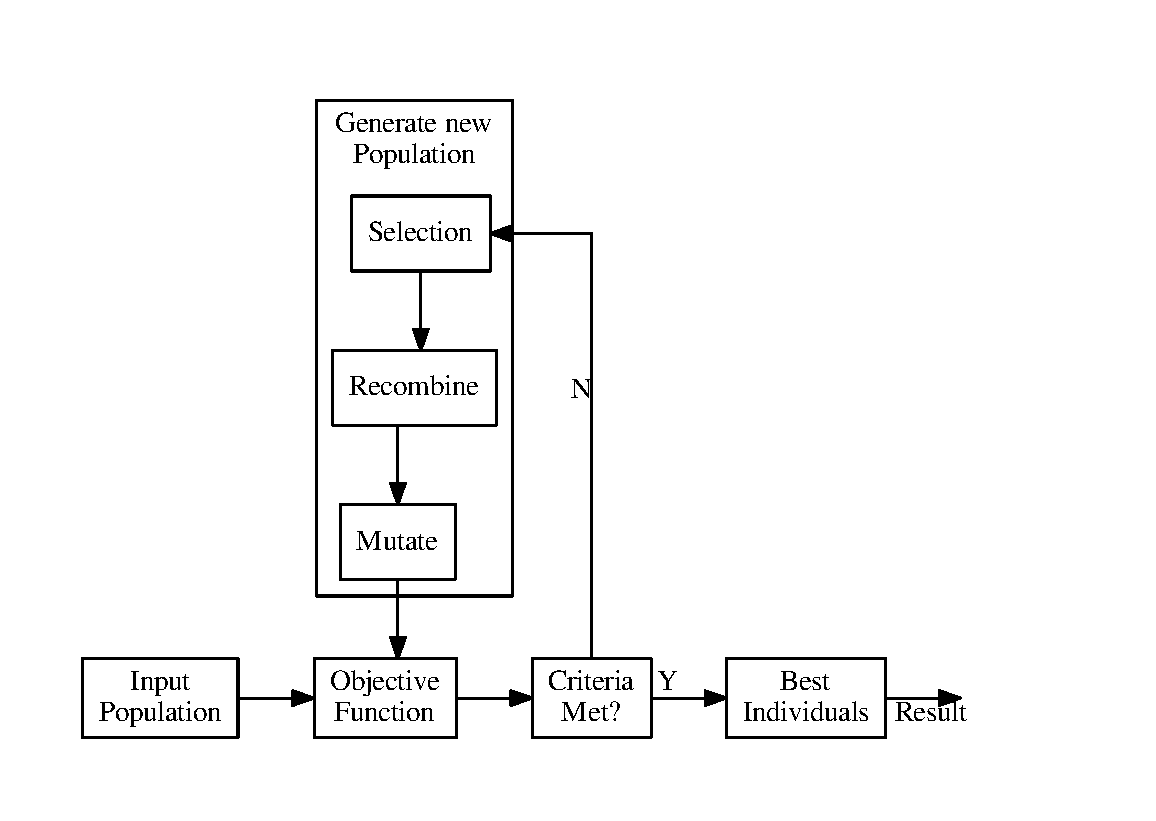
\includegraphics[width=12cm]{ga_ov}
\caption{The basic structure of a genetic algorithm \cite{geatbx}.}
\label{f:ga_ov}
\end{figure}

	Genetic algorithm is an unsupervised exploration technique that attempts to find optimal answers in large problem spaces. 
	Genetic algorithms operate on \emph{chromosomes} which are essentially a vector representation of the problem space.
	An initial population of chromosomes are rated using an \emph{objective} or \emph{fitness} function which determines the quality of each result. 
	If a sufficient answer has been found then the algorithm may quit.
	Otherwise, a new population is generated using selection, recombination and mutation. 
	
	There are many variations on each of these operations. Selection could be as simple as passing on the top $x$ chromosomes and then randomly generating the remainder of the population after each \emph{generation}. 
	Another alternative is tournament selection, where pairs of chromosomes are selected randomly from the population and the higher of the two is passed on to the next generation. 
	Recombination is typically done using the crossover operator which chops two chromosomes at some \emph{gene} location (element index) and swaps the ends.
	Finally mutation randomly modifies a randomly selected gene in a randomly selected chromosome.
	There are many probabilistic parameters that require calibration for each operator as well as the population size and number of generations.
	
	There is not a generally well defined methodology for selecting these parameters. These experiments will evolve a population of size 100 over 30 generations. 80\% of chromosomes are selected from the previous generation using tournament selection. The tournament selection itself passes on the best chromosomes with a probability of 80\%. The crossover rate is 40\% and the mutation rate is 50\%.

\subsection{Two Stage GA}
	The mapping and scheduling algorithm follows the procedure used in \cite{bolchini2013reliability} and \cite{kang2014reliability}. 
	Two stages of genetic algorithms (GA) are used to explore both the techniques used to harden each task and the core assignment for each task and its replicas. 
	The basic flow is shown in Figure~\ref{f:dse}. 
	The GA is implemented using \cite{jgap}.  
	The Reliability Aware (RA) stage is responsible for mapping a fault tolerance mechanism to each task. 
	The RA stage then generates a chromosome structure for the Mapping and Scheduling (MS) stage. 
	The MS stage attempts to find an allocation for each task onto a core that maximizes the average QoS across all modes in the system using the response time anlaysis in Section~\ref{s:mcfts}.
	
\addfigure{0.6}{dse.pdf}{Overview of DSE workflow using nested genetic algorithm searches}{f:dse}
	
	The chromosome in the RA stage has one gene for each task and each gene is an integer representing a fault tolerance mechanism being used in the system. 
	For instance, consider a task set with three HI tasks ${\tau_1,\tau_2,\tau_3}$ being mapped onto a platform that supports LS, DMR and TMR - the chromosome would consist of three genes each limited to integers in the range $[0,2]$. 
	
	The RA fitness function (FF) must determine the fitness (QoS) for each configuration of fault tolerance mechanisms. 
	The FF creates a new task set using the transformations in Table~\ref{t:transform} as well as the necessary constraints. 
	The FF then creates a chromosome template for the MS stage based on the transformed task set. 
	Given the number of processors that a task can be mapped to, $n$, it is possible to determine for each FTM a mapping rule that generates a unique configuration from an integer. 
	Each gene in the chromosome is an integer representing a unique allocation for a task and its replicas. 
	It is important that the task and replicas are represented by a single gene or else most chromosomes will result in illegal configurations after mutation and crossover. 
	Table~\ref{t:mschrom} shows the number of configurations for each type of FTM and how to derive a unique allocation as a function of the number of candidate cores ($n$) from a random integer $x$. 
	The conversion rule provides an index into an ordered list of the cores. After each core is allocated it is removed from the list.
	
	For example, consider a task and two replicas using TMR in a sytem with 5 processing cores. 
	All three tasks must go on different cores. 
	The number of configurations is $5 \cdot 4 \cdot 3 = 60$. 
	The GA will generate a random integer in the range $[0,59]$ representing a unique mapping of the three tasks onto the system, say 47. 
	The number 47 is converted using the TMR rule to $(47/(4\cdot3),(47\bmod(4\cdot3))/3,47\bmod3) = (3,3,1)$. 
	Suppose the core list is $\{\pi_1,\pi_2,\pi_3,\pi_4,\pi_5\}$. 
	The first copy is allocated to $\pi_3$ and $\pi_3$ is then removed from the list. 
	The next copy is assigned to $\pi_4$ (now at index 3) and the third copy is assigned to $\pi_1$. 
	
	\begin{table}
\caption{Rules for generating unique MS configurations from an integer $x$ for $n$ cores}
\label{t:mschrom}
\centering
	\begin{tabular}{@{}l|cc@{}}
	\toprule
	Technique & Configurations & Conversion Rule \\
	\bottomrule
	none & $n$ & $(x)$\\
	LS & $n$ & $(x)$ \\
	DMR & $n(n-1)$ & $(\frac{x}{x-1},x\bmod{x-1})$ \\
	TMR & $n(n - 1)(n-2)$ & $(\frac{x}{(n - 1)(n - 2)}, \frac{x\bmod ((n-1)*(n-2))}{n-2}, x \bmod (n-2))$ \\
	PR & $n^2 (n-1)$ & $(\frac{x}{n(n - 1)}, \frac{x \bmod (n*(n-1))}{n-1}, x \bmod (n-1))$ \\
	\end{tabular}
\end{table} 	

	A unique MS stage is instantiated for each chromosome in the RA stage population. 
	The MS stage creates a schedule based on the chromosome and passes it along to the schedulability analysis. 
	
	
\subsection{Performance Optimization}

	The performance overhead of nesting one lengthy search inside another is problematic. 
	The performance impact was resolved by modifying the RA stage to request a new thread from a pool whenever calling the RA fitness function. 
	Using 20 threads on a 30 core system resulted in significant speedups and makes this a much more practical implementation given sufficient computing resources. 
	We furthermore implement early exiting if a solution is found with perfect QoS or the best QoS has not been improved in four generations.

\subsection{Results}


	Three platforms were tested to verify the mapping: one system (ODR) with four cores using only DMR, the second (LS) with two lockstep cores, and the third (FP) using one lockstep core and two processing cores using DMR. 
	The same task generation algorithm was used as in Section~\ref{s:singlecore-results}. 
	The systems were tested with 100 task sets with between 20 and 40 tasks, half of which were HI, an average utilization of 80\%, and a maximum WCET factor ($C(HI)/C(LO)$) of 3. 
	Note that for the ODR and LS systems, the RA stage could be skipped for efficiency purposes as there is only one available mechanism.

	Any system that is schedulable for one system should be schedulable for all three. 
	They should only differ (possibly) in the QoS of each mode. 
	Furthermore, we expect the QoS of the ODR and FP systems to be higher than that of the LS.  

	Figure~\ref{f:platform-sched} shows the schedulability results for the three platforms. 
	The schedulability of ODR and LS were 69\% and 70\% respectivey. 
	In three cases, the tool failed to find a solution with ODR for a system that passed with LS while only two cases occurred where a LS solution was not found for a system that passed with ODR. 
	The schedulability for the FP platform was 31\% suggesting poor calibration of the GA stages. However, integration with a code generation tool would ideally allow for a very short run time which most recalibrations would significantly extend. 
	Overall, this suggests that the use of genetic algorithms may be a useful starting point but that other semi-random unguided heuristics should also be explored in future work.
	
	Figure~\ref{f:platform-sched} shows the results for average QoS only for task sets successfully scheduled on all three platforms. 
	Here we see that ODR does indeed provide better QoS compared to LS.
	FP provides better QoS in the first three modes compared to LS but not in the HI mode.
	
\addfigure{1}{platform-sched.pdf}{Schedulability results for three different platforms}{f:platform-sched}
\addfigure{1}{platform-qos.pdf}{QoS of the four modes for three different platforms.}{f:platform-qos}

